%%%%%%%%%%%%%%%%%%%%%%%%%%%%%%%%%%%%%%%%%%%%%%%%%%%%%%%%%%%%%%%%%%%%%%%%
%    INSTITUTE OF PHYSICS PUBLISHING                                   %
%                                                                      %
%   `Preparing an article for publication in an Institute of Physics   %
%    Publishing journal using LaTeX'                                   %
%                                                                      %
%    LaTeX source code `ioplau2e.tex' used to generate `author         %
%    guidelines', the documentation explaining and demonstrating use   %
%    of the Institute of Physics Publishing LaTeX preprint files       %
%    `iopart.cls, iopart12.clo and iopart10.clo'.                      %
%                                                                      %
%    `ioplau2e.tex' itself uses LaTeX with `iopart.cls'                %
%                                                                      %
%%%%%%%%%%%%%%%%%%%%%%%%%%%%%%%%%%
%
%
% First we have a character check
%
% ! exclamation mark    " double quote  
% # hash                ` opening quote (grave)
% & ampersand           ' closing quote (acute)
% $ dollar              % percent       
% ( open parenthesis    ) close paren.  
% - hyphen              = equals sign
% | vertical bar        ~ tilde         
% @ at sign             _ underscore
% { open curly brace    } close curly   
% [ open square         ] close square bracket
% + plus sign           ; semi-colon    
% * asterisk            : colon
% < open angle bracket  > close angle   
% , comma               . full stop
% ? question mark       / forward slash 
% \ backslash           ^ circumflex
%
% ABCDEFGHIJKLMNOPQRSTUVWXYZ 
% abcdefghijklmnopqrstuvwxyz 
% 1234567890
%
%%%%%%%%%%%%%%%%%%%%%%%%%%%%%%%%%%%%%%%%%%%%%%%%%%%%%%%%%%%%%%%%%%%
%
\documentclass[12pt]{iopart}
\newcommand{\gguide}{{\it Preparing graphics for IOP Publishing journals}}
%Uncomment next line if AMS fonts required
\usepackage{iopams}  
\usepackage{hyperref}

\usepackage{graphicx}
\usepackage{tikz}
\usepackage{subcaption}
\usepackage{algpseudocode}
\usepackage{algorithm}
\usepackage{stackengine}

\algrenewcommand{\alglinenumber}[1]{\tiny#1:}

\newcommand\specialcaret{%
  \stackengine{0pt}{\ \,}{\scalebox{1.1}[2]{\raisebox{-0.9ex}{\string^}}}{O}{c}{F}{T}{L}}

\begin{document}

\title[Author guidelines for IOP Publishing journals in  \LaTeXe]{Generalized Prefix and Postfix Faultless, Fixed-Depth Grammars in Symbolic Regression}

\author{Content \& Services Team}

\address{IOP Publishing, Temple Circus, Temple Way, Bristol BS1 6HG, UK}
\ead{submissions@iop.org}
\vspace{10pt}
\begin{indented}
\item[]August 2017
\end{indented}

\begin{abstract}
This document describes the  preparation of an article using \LaTeXe\ and 
\verb"iopart.cls" (the IOP Publishing \LaTeXe\ preprint class file).
This class file is designed to help 
authors produce preprints in a form suitable for submission to any of the
journals listed in table~\ref{jlab1} on the next page.  You are not obliged to use this class file---we accept
submissions using all common \LaTeX\ class and style files.  The \verb"iopart.cls"
class file is supplied merely as a convenience for those authors who find it useful.
This document gives both general advice that applies whatever class file you use, and specific advice
that applies if you choose to use \verb"iopart.cls".

We also accept submissions in Word format.  See elsewhere on this site for guidelines on Word submissions.

If you have any queries about this document or any aspect of preparing your article for submission please contact us at the e-mail address given above.
\end{abstract}

%
% Uncomment for keywords
%\vspace{2pc}
%\noindent{\it Keywords}: XXXXXX, YYYYYYYY, ZZZZZZZZZ
%
% Uncomment for Submitted to journal title message
%\submitto{\JPA}
%
% Uncomment if a separate title page is required
%\maketitle
% 
% For two-column output uncomment the next line and choose [10pt] rather than [12pt] in the \documentclass declaration
%\ioptwocol
%



\section{Introduction}
Symbolic regression (SR) typically denotes the process of finding a symbolic model $f\left(\vec{x}\right)$ that takes an $N$-dimensional feature vector $\vec{x}$ as input and outputs a value $f\left(\vec{x}\right)$ denoting a prediction of the label $y$, such that some user-defined loss metric $\mathcal{L}\left(f\left(\vec{x}\right),y\right)$ is minimized. Usually, the symbolic models constituting the search space contain ``tokens'', i.e., nodes, in one of the following classes:
\begin{itemize}
\item[--] Leaves: Usually, any of the individual features $\vec{x} = \{x_1, x_2, \ldots,x_{N}\}$ and a constant token that can be optimized with some non-linear optimization routine like L-BFGS \cite{doi:10.1137/0916069} or Levenberg-Marquadt \cite{83b09f23-b20e-3617-8f72-24765b713f7b} \cite{doi:10.1137/0111030}.
\item[--] Unary operators: Usually any operator that takes 1 real argument as input and outputs a real number, such as $\cos$, $\sin$, $\exp$, $\ln$, $\tan$, etc.
\item[--] Binary operators: Usually any operator that takes 2 real arguments as input and outputs a real number, such as $+$, $-$, $*$, $\div$, etc.
\end{itemize}
\subsection{Symbolic Regression Algorithms}
To the best of our knowledge, the only paper that studies the effect of prefix vs postfix expression representations on symbolic regression convergence is \cite{hemberg2008pre}.  In \cite{hemberg2008pre}, the authors compare prefix, infix, and postfix notation-based grammars on 5 bivariate symbolic regression benchmarks and found a greater relative performance of the postfix grammar that increased with complexity of ground-truth expressions. 
However, this performance difference was mostly due to the smaller percentage of invalid individuals generated with the postfix grammar compared to the prefix grammar.  
Furthermore, we note 2 main limitations of this result for its applicability to modern prefix/postfix-based Symbolic Regression software which motivate this paper:
\begin{enumerate}
\item The study does not consider \emph{faultless grammars}, i.e., grammars which do not produce invalids.
\item The study only considers genetic algorithm for symbolic regression and does not explore other symbolic regression algorithms/search strategies. 
\end{enumerate}
In this paper, we document faultless grammars for generating fixed-depth prefix and postfix expressions. Additionally we analyse and compare the performance of various algorithms on standard symbolic regression benchmarks when using these grammars, namely, Random Search (as a baseline), Monte Carlo Tree Search (MCTS), Particle Swarm Optimization (PSO), Genetic Programming (GP), and Simualted Annealing (SA). 
\par Other papers such as \cite{lacava2021contemporary}, \cite{10.1145/3205455.3205539}, and \cite{Zegklitz2021} have documented comprehensive comparisons of different symbolic regression methods. However, such comparisons are almost always within the context of different frameworks, which can potentially obscure an otherwise very good algorithm by differences in implementation efficiency/speed. Therefore, we implement all the algorithms and grammars in one common framework, namely, a C++ framework utilizing the Eigen template library  \cite{eigenweb} for fast matrix computations and non-linear constant optimization, \href{https://github.com/edfink234/Alpha-Zero-Symbolic-Regression/tree/prefix_and_postfix_cpp_implementation}{here}.

 

\section{Background}\label{sec:Background}

At the core of every symbolic regression framework lies an underlying choice of expression representation.
As an example, Table \ref {GECCO_Framework_reps} denotes the list of frameworks considered in the ``Interpretable Symbolic Regression for Data Science: Analysis of the 2022 Competition'' \cite{defranca2023interpretable} and the main underlying expression representations utilized. 

\begin{table}
\caption{\label{GECCO_Framework_reps}List of Symbolic Regression Frameworks submitted to the 2022 Genetic and Evolutionary Computation Conference competition \cite{defranca2023interpretable}, their underlying expression representations, and if the expression representation was stated directly in the cited paper or implied via source code and/or references. 
\\ The frameworks Bingo, E2E Transformer, QLattice, and Operon state their choice of expression representation directly in the cited papers (namely \cite{10.1145/3520304.3534031}, \cite{kamienny2022endtoend}, \cite{Brolos2021AnAT}, and \cite{10.1145/3377929.3398099}, respectively). PS-Tree does not specify \cite{zhang2022ps} but they use the Deap GP framework \cite{DEAP_JMLR2012} (see \href{https://github.com/hengzhe-zhang/PS-Tree/blob/master/pstree/common\_utils.py\#L4}{here}) which represents expressions with prefix notation. TaylorGP strongly implies prefix notation in the example expression written in section 4.1.1 of their paper \cite{10.1145/3512290.3528757}. In Table 2 of the EQL Paper \cite{pmlr-v80-sahoo18a} they refer to the expressions as ``random graphs,'' and evidence of their acyclicity is given in their Jupyter notebook \href{https://github.com/martius-lab/EQL/blob/master/EQL-DIV-ICML-Python3/Evaluation.ipynb}{here}. GeneticEngine implies prefix usage in section 3.2 of their paper \cite{10.1145/3564719.3568697} (namely, ``Starting with the non-terminal root type $\ldots$''). PySR does not state the expression representation in their paper \cite{cranmer2023interpretable}, but a pre-order traversal of the expression tree is somewhat implied in the Julia source file \href{https://github.com/MilesCranmer/SymbolicRegression.jl/blob/db476a708762c81f46f27f22751f7ff3d1153dc7/src/Equation.jl}{here}. The uDSR framework states pre-order traversal of expression trees for the DSR component in their paper (namely, ``$\ldots$ in the pre-order (depth-first then left-to-right) traversal of the corresponding \emph{expression tree} $\ldots$'' in section 2), and for the GP expression generation, use of the Deap GP framework is shown \href{https://github.com/dso-org/deep-symbolic-optimization/blob/2069d4eda47b0fd6d3e66e0ade9605cd9574b87c/dso/dso/gp/utils.py\#L10}{here} \cite{NEURIPS2022_dbca58f3}. 
$\mathrm{GP}_{\mathrm{ZGD}}$ \cite{10.1145/3377930.3390237} somewhat implies a pre-order traversal of expression trees in the C source file \href{https://github.com/grantdick/gpzgd/blob/42e5a1829a0b8a2eb50e116000001f82c770791e/src/gp.c}{here}. NSGA-DCGP states at the beginning of section 2 that ``To represent our functional programs we use the Cartesian Genetic Programming framework,'' \cite{izzo2016differentiable}  and the paper they cite directly states ``In CGP, programs are represented in the form of directed acyclic graphs'' \cite{Miller2011}.} 
\begin{tabular*}{\textwidth}{lll} %open PhD_Papers/2304.01117.pdf 
\br
Framework&Expression Representation & Stated Directly or Implied\\
\mr
Bingo \cite{10.1145/3520304.3534031} &Acyclic Graph & Stated Directly\\ %Specified in Paper
E2E Transformer \cite{kamienny2022endtoend} &prefix & Stated Directly\\ %Specified in Paper
PS-Tree \cite{zhang2022ps} &prefix & Implied \\ %Not directly specified in Paper, but they use Deap GP (see here: https://github.com/hengzhe-zhang/PS-Tree/blob/master/pstree/common_utils.py#L4) which uses prefix notation internally (Simone said so)
QLattice \cite{Brolos2021AnAT} & Acyclic Graph & Stated Directly\\ %Specified in Paper
TaylorGP \cite{10.1145/3512290.3528757} & prefix & Implied \\ %Not directly specified, but they strongly imply it by writing examples in prefix notation in section 4.1.1 of the paper here: https://arxiv.org/pdf/2205.09751.pdf
EQL \cite{pmlr-v80-sahoo18a} & Acyclic Graph & Implied\\%Table 2 refers to the expressions as ``random graphs,'' and the following Jupyter notebook gives further evidence for this: https://github.com/martius-lab/EQL/blob/master/EQL-DIV-ICML-Python3/Evaluation.ipynb
GeneticEngine \cite{10.1145/3564719.3568697} & prefix & Implied \\ %'' Starting with the non-terminal
%root type, a concrete subclass is non-deterministically selected, and that object is created. For each field (or constructor argument), a compatible object is constructed by recursively calling this algorithm. The base case is when native
%types (like int or float) are used, and then native random
%value generators are used.'' (section 3.2 ``Meta-handlers'')  
Operon \cite{10.1145/3377929.3398099} & postfix  & Stated Directly \\ %Specified in Paper
PySR \cite{cranmer2023interpretable} & prefix & Implied \\%Very characteristic Pre-order traversal of Binary Tree: https://github.com/MilesCranmer/SymbolicRegression.jl/blob/db476a708762c81f46f27f22751f7ff3d1153dc7/src/Equation.jl
uDSR \cite{NEURIPS2022_dbca58f3} & prefix & Implied \\ %For the DNN part it is stated ``in the pre-order (depth-first then left-to-right) traversal of the corresponding expression'' and the GP part uses deap (see here: https://github.com/dso-org/deep-symbolic-optimization/blob/2069d4eda47b0fd6d3e66e0ade9605cd9574b87c/dso/dso/gp/utils.py#L10)
$\mathrm{GP}_{\mathrm{ZGD}}$ \cite{10.1145/3377930.3390237} & prefix & Implied\\ %Implied, as init_tree builds expressions by adding operators further down (pre-order) and connects the new pointer by pointing the parent to the current tree
NSGA-DCGP \cite{izzo2016differentiable} & Acyclic Graph & Implied \\%``To represent our functional programs we use the Cartesian Genetic Programming framework'' which states ``In CGP, programs are represented in the form of directed acyclic graphs'' \cite{Miller2011}
\br
\end{tabular*}
\end{table}

As one can see in Table \ref{GECCO_Framework_reps}, the majority of frameworks represent expressions through a pre-order traversal of expression trees, followed by acyclic graph representations and lastly postfix notation.
Figure \ref{fig:pub_freqs_pre_post_acyc_graph} shows a histogram of publication frequencies mentioning these representations in the context of symbolic regression throughout the years, obtained with the help of the scholarly python module \cite{cholewiak2021scholarly}.  %code here: 

\begin{figure}
    \centering
    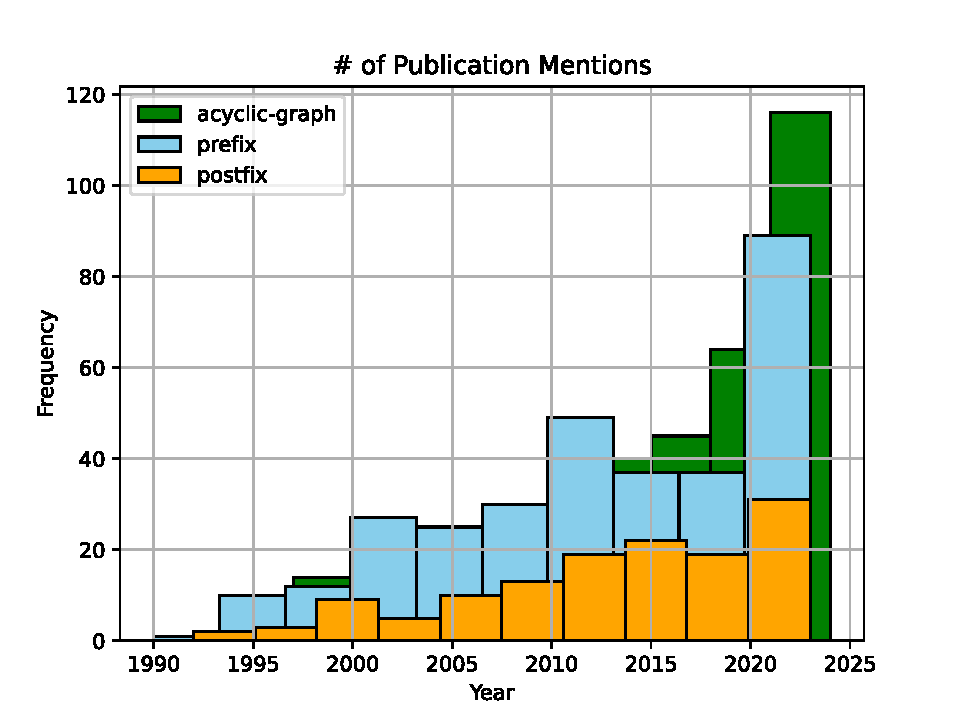
\includegraphics[width=\linewidth]{pub_freqs.pdf}
    \caption{Number of mentions of prefix, postfix, and acyclic graph in publications pertaining to symbolic regression. The python module scholarly was used to generate this histogram \cite{cholewiak2021scholarly}. The search queries utilized were ``postfix notation'' AND ``symbolic regression'', ``prefix notation'' AND ``symbolic regression'', ``acyclic graph'' AND ``symbolic regression'', ``reverse polish notation'' AND ``symbolic regression'', ``polish notation'' AND ``symbolic regression'', and ``acyclic-graph'' AND ``symbolic regression''. The script to reproduce this plot is \href{https://github.com/edfink234/Alpha-Zero-Symbolic-Regression/blob/2999916868007841f05c272498edef3aa2dcb494/Figure_1/notations_pubs_counter.py}{here}.} 
    \label{fig:pub_freqs_pre_post_acyc_graph}
\end{figure}

It can be seen that the preferred choice of expression representation tends to be either prefix notation or acyclic graphs, and postfix tends to not be preferred as much. A possible explanation for the preference is that starting an expression from the root node, as is typically the case for prefix and acyclic graph-based expression representations, lends itself to a natural termination condition, i.e., when all of the branches from the root node terminate at a leaf node. Acyclic graphs have the added advantage of allowing children nodes to have mulitple parents, reducing the memory necessary to represent symbolic expressions with identical sub-components when compared to trees. On the other hand, postfix expressions imply building an expression tree from the leaf nodes; thus, there exist nodes where the expression tree can be either terminated or expanded further up using the same postfix-grammar. 

In this paper, we restrict the analysis to prefix and postfix notations, as these can be easily represented with the same underlying data-structure, though acyclic-graph grammars can be an analysis for future work. Furthermore, the methods developed in this paper assume expressions are represented as an array of tokens. In this schema, a representation of an arbitrary acyclic graph expression is not readily apparent.


\subsection{Prefix and Postfix}
Using prefix notation for symbolic regression entails building an expression starting from a root node, i.e., an operator. Postfix notation, on the other hand, begins building the expression from leaf nodes. Figure \ref{fig:prefix_vs_postfix} illustrates the difference.


\begin{figure}
    \begin{subfigure}[b]{0.51\textwidth}
        \centering
        \begin{tikzpicture}
            \node[text width = 6 cm, align = center] at (0,0) {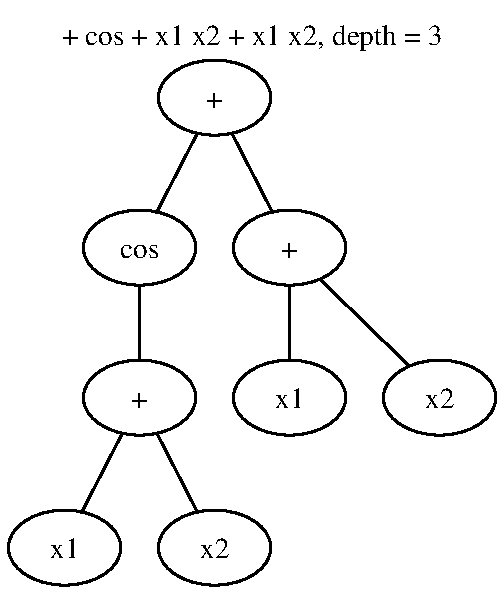
\includegraphics[width=\linewidth, keepaspectratio]
            {expression_tree_PN.pdf}};
            \node at (-1.35, 2.4) {\textcolor{red}{\textbf{1}}};
            \node at (-2.25, 0.6) {\textcolor{red}{\textbf{2}}};
            \node at (-2.25, -1.2) {\textcolor{red}{\textbf{3}}};
            \node at (-3.15, -3) {\textcolor{red}{\textbf{4}}};
            \node at (-1.325, -3) {\textcolor{red}{\textbf{5}}};
            \node at (-0.4, 0.6) {\textcolor{red}{\textbf{6}}};
            \node at (-0.4, -1.2) {\textcolor{red}{\textbf{7}}};
            \node at (1.4, -1.2) {\textcolor{red}{\textbf{8}}};
        \end{tikzpicture}
        \caption{prefix}
        \label{subfig:prefix_tree_example}
    \end{subfigure}
    \hspace{1cm}
    \begin{subfigure}[b]{0.51\textwidth}
        \centering
        \begin{tikzpicture}
            \node[text width = 6 cm, align = center] at (0,0) {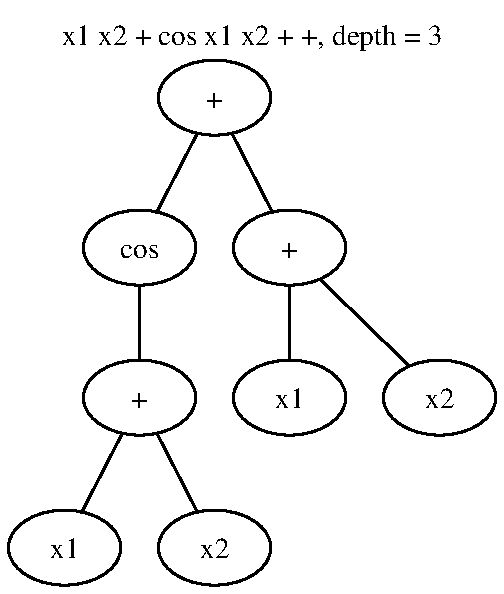
\includegraphics[width=\linewidth, keepaspectratio]{expression_tree_RPN.pdf}};
            \node at (-1.35, 2.4) {\textcolor{red}{\textbf{8}}};
            \node at (-2.25, 0.6) {\textcolor{red}{\textbf{4}}};
            \node at (-2.25, -1.2) {\textcolor{red}{\textbf{3}}};
            \node at (-3.15, -3) {\textcolor{red}{\textbf{1}}};
            \node at (-1.325, -3) {\textcolor{red}{\textbf{2}}};
            \node at (-0.4, 0.6) {\textcolor{red}{\textbf{7}}};
            \node at (-0.4, -1.2) {\textcolor{red}{\textbf{5}}};
            \node at (1.4, -1.2) {\textcolor{red}{\textbf{6}}};
        \end{tikzpicture}
        \caption{postfix} \label{subfig:postfix_tree_example}
    \end{subfigure}
    \caption{Prefix (left) vs postfix (right) representation of the infix expression $f(x_1, x_2) = \cos(x_1 + x_2) + (x_1 + x_2)$. The numbers \textcolor{red}{\textbf{1}} - \textcolor{red}{\textbf{8}} denote the order of tokens. The postfix expression is given by the post-order traversal of the tree, whereas the prefix expression is obtained by the pre-order traversal of the tree.}
    \label{fig:prefix_vs_postfix}
\end{figure}

\par One major difference between the two methods of building expressions is that, for prefix notation, once an expression tree branch is complete, it cannot be expanded further \emph{down} without a mutation/substitution of a leaf node. On the other hand, for postfix notation, one can continue expanding the expression tree further \emph{up} starting from the root node; an example is shown in Figure \ref{fig:postfix_add_1}.

\begin{figure}
    \begin{subfigure}[b]{0.51\textwidth}
        \centering
        \begin{tikzpicture}
            \node[text width = 6 cm, align = center] at (0,0) {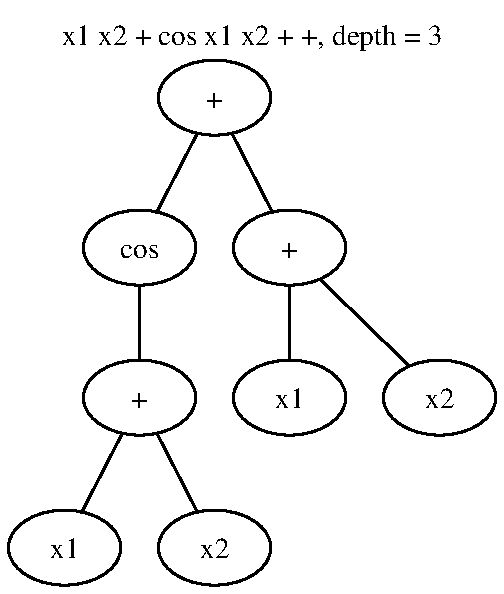
\includegraphics[width=\linewidth, keepaspectratio]{expression_tree_RPN.pdf}};
            \node at (-1.35, 2.4) {\textcolor{red}{\textbf{8}}};
            \node at (-2.25, 0.6) {\textcolor{red}{\textbf{4}}};
            \node at (-2.25, -1.2) {\textcolor{red}{\textbf{3}}};
            \node at (-3.15, -3) {\textcolor{red}{\textbf{1}}};
            \node at (-1.325, -3) {\textcolor{red}{\textbf{2}}};
            \node at (-0.4, 0.6) {\textcolor{red}{\textbf{7}}};
            \node at (-0.4, -1.2) {\textcolor{red}{\textbf{5}}};
            \node at (1.4, -1.2) {\textcolor{red}{\textbf{6}}};
        \end{tikzpicture}
        \caption{postfix (before)}
    \end{subfigure}
    \hspace{1cm}
    \begin{subfigure}[b]{0.51\textwidth}
        \centering
        \begin{tikzpicture}
            \node[text width = 6 cm, align = center] at (0,0) {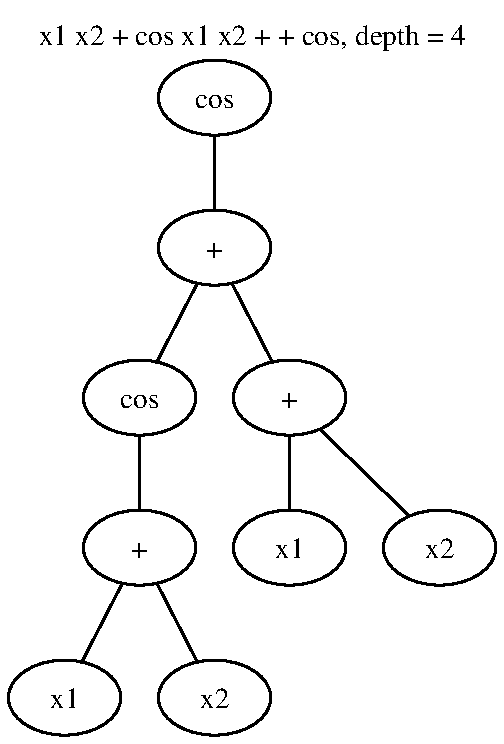
\includegraphics[width=\linewidth, keepaspectratio]{expression_tree_1_RPN.pdf}};
            \node at (-1.35, 3.3) {\textcolor{red}{\textbf{9}}};
            \node at (-1.35, 1.5) {\textcolor{red}{\textbf{8}}};
            \node at (-2.25, -0.3) {\textcolor{red}{\textbf{4}}};
            \node at (-2.25, -2.1) {\textcolor{red}{\textbf{3}}};
            \node at (-3.15, -3.9) {\textcolor{red}{\textbf{1}}};
            \node at (-1.325, -3.9) {\textcolor{red}{\textbf{2}}};
            \node at (-0.4, -0.3) {\textcolor{red}{\textbf{7}}};
            \node at (-0.4, -2.1) {\textcolor{red}{\textbf{5}}};
            \node at (1.4, -2.1) {\textcolor{red}{\textbf{6}}};
        \end{tikzpicture}
        \caption{postfix (after)}
    \end{subfigure}
    \caption{Adding a node (right) to a postfix expression tree (left, node \textcolor{red}{\textbf{9}}). As one can see, even though the expression on the left is complete, the tree can grow using the same method. This is not the case for the prefix representation. For example, to continue the expression tree in Figure \ref{subfig:prefix_tree_example}, one would have to add nodes going up from the root.}
    \label{fig:postfix_add_1}
\end{figure}

\subsection{Building Fixed-Depth Expressions}
Building fixed-depth expressions using either prefix or postfix notation requires determining the set of legal nodes at each step. 
\par Each step corresponds to adding a ``token'' to the current expression list. The set of nodes that can be selected at a given step is defined such that any possible \emph{valid} expression can eventually be generated with depth $N$ (an input parameter). The tokens are selected and appended to an expression list in the left-to-right order that they appear in the prefix or postfix notations; see e.g. the titles of Figures \ref{subfig:prefix_tree_example} and \ref{subfig:postfix_tree_example}, respectively. 
\par The set of legal tokens at each step is determined by the following formula \ref{eq:Generic_Policy_Mask}

\begin{equation}
    \vec{\pi}_{\mathrm{mask}} \left(\vec{U}_{A}, \vec{B}_{A}, \vec{L}_{A}\right) = 
\vec{U}_{A}  + \vec{B}_{A} +\vec{L}_{A},
\label{eq:Generic_Policy_Mask}
\end{equation}

where $\vec{U}_{A}$, $ \vec{B}_{A}$, and $\vec{L}_{A}$ correspond to the set of allowed unary operators, binary operators, and leaves, respectively. Additionally, let $N_U$, $N_B$, $N_L$ denote the number of considered unary operators, binary operators, and leaves, respectively,  and $N_{T}$ shall denote the total number of tokens considered.

Determining whether a unary node, binary node, and/or a leaf node is allowed at the current step differs depending on if the expression is represented using prefix or postfix notation. The specific rules are thus explained in the remainder of this section.

\subsection{Prefix Grammar}\label{subsec:prefix_grammar}
At the first step, the only allowed tokens are the set of all considered operators of size $N_U + N_B$, unless the specified depth $N=0$, in which case, building the expression entails only one step, namely, selecting a leaf node.
\par At each subsequent step, the set of allowed tokens are determined as follows:
\subsubsection{Unary Operators}
We say any token in the set of all considered unary operators is valid if adding a unary operator to the current expression can result in an expression with depth less than or equal to the specified depth $N$. If this condition is false, then a unary operator is not allowed.
\subsubsection{Binary Operators}
We say any token in the set of all considered binary operators is valid if adding a binary operator to the current expression can result in an expression with depth less than or equal to the specified depth $N$. If this condition is false, then a binary operator is not allowed.
\subsubsection{Leaf Nodes}
We say any token in the set of all considered leaf nodes is valid if \emph{both} of the following conditions are false for the current expression:
\begin{enumerate}
    \item The number of leaf nodes in the current expression is equal to the number of binary nodes in the current expression minus 1.
    \item Adding a leaf node results in the minimum depth of the expression being less than the desired depth $N$ \textbf{and} the number of leaf nodes in the current expression is equal to the number of binary nodes in the current expression.
\end{enumerate}


\subsection{Postfix Grammar}\label{subsec:postfix_grammar}
At the first step, the only allowed tokens are the leaf nodes of size $N_L$.
\par At each subsequent step, the set of allowed tokens are determined as follows:
\subsubsection{Unary Operators}
We say any token in the set of all considered unary operators is valid if the number of leaf nodes in the current expression is greater than or equal to 1 \textbf{and} if adding a unary operator to the current expression can result in an expression with depth less than or equal to the specified depth $N$. If this condition is false, then a unary operator is not allowed.
\subsubsection{Binary Operators}
We say any token in the set of all considered binary operators is valid if the number of binary nodes in the current expression is \textbf{not} equal to the number of leaf nodes in the current expression minus 1. If this condition is false, then a binary operator is not allowed.
\subsubsection{Leaf Nodes}
We say any token in the set of all considered leaf nodes is valid if adding a leaf node results in the minimum depth of the expression being less than or equal to the desired depth $N$. If this condition is false, then a leaf node is not allowed.

\subsection{Conclusion}
What can be seen from sections \ref{subsec:prefix_grammar} and \ref{subsec:postfix_grammar} is that the grammar for building postfix expressions is less complicated than the grammar for building prefix expressions. The main reason for this difference is that, in prefix notation, one must ensure the expression does not complete until it reaches the desired depth $N$. On the other hand, postfix notation imparts the ability to add nodes to an RPN expression \emph{indefinitely} without change of method; this is not the case for prefix notation. \par Determining the minimum depth and completeness of a prefix or postfix expression list of tokens can be done via a stack-based approach as shown in algorithms \ref{alg:getPNdepth} and \ref{alg:getRPNdepth}.

\begin{algorithm}
\scriptsize
\caption{Calculate Depth and Completeness of \textbf{Polish Notation (PN)} expressions. Algorithm from \cite{77180279}.}
\label{alg:getPNdepth}
\hspace*{\algorithmicindent} \textbf{input:}  expression, expression list of tokens in prefix notation \\
\hspace*{\algorithmicindent} \textbf{output:} Depth of expression\\
\hspace*{\algorithmicindent} \textbf{output:} If expression is complete 
\begin{algorithmic}[1] 
\Function{getPNdepth}{expression}  %code here
    \If{expression is empty}
        \State \Return 0, \textbf{False}
    \EndIf

    \State Initialize empty stack
    \State Initialize depth, numBinary, and numLeaves to 0

    \For{token \textbf{in} expression}
        \If{token is binary operator}
            \State Push 2 onto stack   \Comment\texttt{{Number of operands for binary operators}}
            \State numBinary $\gets$ numBinary+1
        \ElsIf{token is unary operator} 
            \State Push 1 onto stack  \Comment\texttt{{Number of operands for unary operators}}
        \Else  \Comment\texttt{{An operand}}
            \State numLeaves $\gets$ numLeaves+1
            \While{stack is not empty \textbf{and} top of stack == 1}
                \State Pop top of stack \Comment\texttt{{Remove fulfilled unary operators}}
            \EndWhile
            \If{stack is not empty}
                \State Decrement top of stack by 1 \Comment\texttt{{Indicate operand is consumed}}
            \EndIf
        \EndIf
        \State  depth $\gets$ max(depth, stack length + 1)
    \EndFor
    \State \Return depth - 1, numLeaves == numBinary + 1 
\EndFunction
\end{algorithmic}
\end{algorithm}

\begin{algorithm}
\scriptsize
\caption{Calculate Depth and Completeness of \textbf{Reverse Polish Notation (RPN)} expressions.  Algorithm from \cite{77128902}.}
\label{alg:getRPNdepth}
\hspace*{\algorithmicindent} \textbf{input:}  expression, expression list of tokens in postfix notation \\
\hspace*{\algorithmicindent} \textbf{output:} Depth of expression\\
\hspace*{\algorithmicindent} \textbf{output:} If expression is complete 
\begin{algorithmic}[1]
\Function{getRPNdepth}{expression} %code here
    \If{expression is empty}
        \State \Return 0, \textbf{False}
    \EndIf

    \State Initialize empty stack

    \For{token \textbf{in} expression}
        \If{token is unary operator} \Comment\texttt{{All unary operators}}
            \State Increment top of stack by 1 
        \ElsIf{token is binary operator} \Comment\texttt{{All binary operators}}
            \State Push max(stack.pop(), stack.pop()) + 1 onto stack 
        \Else  \Comment\texttt{{All operands}}
            \State Push 1 onto stack
        \EndIf
    \EndFor

   \If{size of stack greater than 1}

	    \While{size of stack greater than 1}
	        \State Push max(stack.pop(), stack.pop()) + 1 onto  stack
	    \EndWhile
 	\State \Return stack.pop() - 1, \textbf{False}
    
    \Else
    	\State \Return stack.pop() - 1, \textbf{True}
    	    \EndIf
\EndFunction
\end{algorithmic}
\end{algorithm}

In the next section, the symbolic regression algorithms utilized in this paper are explained in the context of the fixed-depth grammars developed in this section.

\section{Symbolic Regression Algorithms}\label{sec:SymbolicRegressionAlgorithms}

In this section, the fixed-depth implementations of the algorithms we consider in this paper, namely, Random Search, Monte Carlo Tree Search (MCTS), Particle Swarm Optimization (PSO), Genetic Programming (GP), and Simualted Annealing (SA), are explained in detail.

\subsection{Random Search}\label{subsec:RandomSearch}

Random Search is the brute-force approach to symbolic regression.  As a search strategy, brute force has gained increasing attention in recent years \cite{Heule2017TheSO}. For symbolic regression, exhaustive search can rival genetic programming when used with a sufficienctly restrictive grammar \cite{Kammerer2020}.
Our random-search approach is as follows:
\par First, one starts with an empty expression list. Then, while the current expression list is incomplete with depth less than $N$, a random token from the set of legal tokens is appended to the current expression list. When the expression list is complete and has depth $N$, 5 iterations of Levenberg-Marquadt are performed to optimize all of the constant tokens (if any) in the expression. Finally, the parameter values are cached for future use as initial seeds in case the depth-$N$ expression is encountered again during the search. If the expression was not encountered before, all of the constant parameters to be optimized are initially set to 1. After constant optimization, the score of the expression is computed as:

\begin{equation}
\mathrm{Score} = \frac{1}{1+ 1/N_{\mathrm{dat}}\left|\left|\hat{Y}-\vec{Y}\right|\right|^2}, \label{eq:score_formula}
\end{equation}

where $N_{\mathrm{dat}}$ is the number of data points, $\hat{Y}$ are the predicted labels from the expression, $\vec{Y}$ are the true labels, and $0 \leq \mathrm{Score} \leq 1$. 

\par The set of legal tokens is determined using the rules in sections \ref{subsec:prefix_grammar} and \ref{subsec:postfix_grammar}. These rules require determing the minimum depth and completeness of the current expression list. It can be advantages for larger $N$ to cache the results of the depth computations since they will otherwise involve unneccessary repeat-calculations for all subsequent steps of the expression generation. Caching reduces the number of depth computations from $\mathcal{O}(m!)$ to $\mathcal{O}(m)$, where $m$ is the number of tokens in the completed expression. The algorithms for computing the expression depth with caching are tabulated in algorithms \ref{alg:getPNdepth_cache} and \ref{alg:getRPNdepth_cache}. The for-loop required in algorithms \ref{alg:getPNdepth} and \ref{alg:getRPNdepth} is replaced with a single operation per token that is added to the expression list. 

\begin{algorithm}
\scriptsize
\caption{Calculate Depth and Completeness of \textbf{Polish Notation (PN)} expressions with caching. Original algorithm from \cite{77180279}.}
\label{alg:getPNdepth_cache}
\hspace*{\algorithmicindent} \textbf{input:}  expression, expression list of tokens in prefix notation \\
\hspace*{\algorithmicindent} \textbf{input:}  modify, if params should be modified \\
\hspace*{\algorithmicindent} \textbf{input:}  binary, if depth \& completeness should be determined with binary op.  \\
\hspace*{\algorithmicindent} \textbf{input:}  unary, if depth \& completeness should be determined with unary op.  \\
\hspace*{\algorithmicindent} \textbf{input:} leaf, if depth \& completeness should be determined with leaf node \\
\hspace*{\algorithmicindent} \textbf{output:} Depth of expression\\
\hspace*{\algorithmicindent} \textbf{output:} If expression is complete \\
\hspace*{\algorithmicindent} \textbf{param:} stack, the stack used in the algorithm \\
\hspace*{\algorithmicindent} \textbf{param:} idx, the index of the expression element to use in the computation\\
\hspace*{\algorithmicindent} \textbf{param:} numBinary, the number of binary operators in the expression \\
\hspace*{\algorithmicindent} \textbf{param:} numLeaves, the number of leaf nodes in the expression 
\begin{algorithmic}[1]

\Function{getPNdepth}{expression, modify = \textbf{False},  binary = \textbf{False},  unary = \textbf{False},  leaf = \textbf{False}}  %code here
    \If{expression is empty}
        \State \Return 0, \textbf{False}
    \EndIf

    \If{not modify} \Comment\texttt{{called when determining legal tokens}}
        \If{binary}  %\Comment\texttt{{depth, completeness of PN expression + binary op.}}
            \State \Return max(depth, stack length + 2) -1,  numLeaves == numBinary + 2
         \ElsIf{unary}  %\Comment\texttt{{depth, completeness of PN expression + unary op.}}
            \State \Return max(depth, stack length + 2) -1,  numLeaves == numBinary + 1
         \ElsIf{leaf}  %\Comment\texttt{{depth, completeness of PN expression + leaf node}}
            \State lastIdxNot1 $\gets$ index of last element in stack $\neq$ 1
            \State \Return max(depth, lastIdxNot + 1) -1,  numLeaves == numBinary
        \EndIf
    \Else \Comment\texttt{{called after legal token selected}}
        \If{expression[idx] is binary operator}
            \State Push 2 onto stack   \Comment\texttt{{Number of operands for binary operators}}
            \State numBinary $\gets$ numBinary+1
        \ElsIf{expression[idx] is unary operator} 
             \State Push 1 onto stack  \Comment\texttt{{Number of operands for unary operators}}
        \Else  \Comment\texttt{{An operand}}
            \State numLeaves $\gets$ numLeaves+1
            \While{stack not empty \textbf{and} top of stack is 1}
                \State Pop top of stack \Comment\texttt{{Remove fulfilled unary operators}}
            \EndWhile
            \If{stack not empty}
                \State Decrement top of stack by 1 \Comment\texttt{{Indicate operand is consumed}}
            \EndIf
        \EndIf
        \State  depth $\gets$ max(depth, stack length + 1)
        \State idx $\gets$ idx + 1
    \EndIf
    \State \Return depth - 1, numLeaves == numBinary + 1 
\EndFunction
\end{algorithmic}
\end{algorithm}

\begin{algorithm}
\scriptsize
\caption{Calculate Depth and Completeness of \textbf{Reverse Polish Notation (RPN)} expressions with caching.  Original algorithm from \cite{77128902}.}
\label{alg:getRPNdepth_cache}
\hspace*{\algorithmicindent} \textbf{input:}  expression, list of tokens in postfix notation \\
\hspace*{\algorithmicindent} \textbf{input:}  modify, if params should be modified \\
\hspace*{\algorithmicindent} \textbf{input:}  unary, if depth \& completeness should be determined with unary op.  \\
\hspace*{\algorithmicindent} \textbf{input:} leaf, if depth \& completeness should be determined with leaf node \\
\hspace*{\algorithmicindent} \textbf{output:} Depth of expression\\
\hspace*{\algorithmicindent} \textbf{output:} If expression is complete \\
\hspace*{\algorithmicindent} \textbf{param:} stack, the stack used in the algorithm \\
\hspace*{\algorithmicindent} \textbf{param:} idx, the index of the expression element to use in the computation
\begin{algorithmic}[1]
\Function{getRPNdepth}{expression, modify = \textbf{False}, unary = \textbf{False},  leaf = \textbf{False}}  %code here
    \If{expression is empty}
        \State \Return 0, \textbf{False}
    \EndIf

    \If{not modify} \Comment\texttt{{called when determining legal tokens}}
        \If{unary}  %\Comment\texttt{{depth, completeness of RPN expression + unary op.}}
            \If{stack size is 1}
                \State \Return stack[-1], \textbf{True}
            \Else
                \State currMax $\gets$ max(stack[-1]+1,stack[-2])+1
                \For{i $\gets$ stack size - 2 to 1}
                    \State currMax $\gets$ max(currMax,stack[i-1])+1
                \EndFor
                \State \Return currMax - 1, \textbf{False}
            \EndIf
        \ElsIf{leaf}  %\Comment\texttt{{depth, completeness of RPN expression + leaf node}}
            \If{stack is empty}
                \State \Return 0, \textbf{True}
            \Else
                \State currMax $\gets$ max(stack[-1],1)+1
                \For{i $\gets$ stack size - 1 to 1}
                    \State currMax $\gets$ max(currMax,stack[i-1])+1
                \EndFor
                \State \Return currMax - 1, \textbf{False}
            \EndIf
                
        \EndIf

    \Else \Comment\texttt{{called after legal token selected}}
        \If{expression[idx] is binary operator}
            \State Push max(stack.pop(), stack.pop()) + 1 onto stack 
        \ElsIf{expression[idx] is unary operator}
            \State Increment top of stack by 1 
        \Else 
            \State Push 1 onto stack
         \EndIf 
         \State idx $\gets$ idx + 1
         \If{stack size is 1}

             \State \Return stack[-1], \textbf{True}
        \Else
            \State currMax $\gets$ max(stack[-1]+1,stack[-2])+1
            \For{i $\gets$ stack size - 2 to 1}
                \State currMax $\gets$ max(currMax,stack[i-1])+1
            \EndFor
            \State \Return currMax - 1, \textbf{False}
        \EndIf

    \EndIf
\EndFunction
\end{algorithmic}
\end{algorithm}

\subsection{Monte Carlo Tree Search}\label{subsec:MonteCarlo TreeSearch}

Monte Carlo Tree Search (MCTS) has garnered widespread adaptation in game-playing and reinforcement-learning applications \cite{Silver2016} \cite{Swiechowski2023}. MCTS utilizes a combination of random exploration and greedy decision-making to navigate large state spaces by informatively expanding and selecting branches \cite{Swiechowski2023}. This simulative process allows MCTS to gather statistics about the performance of different actions and gradually refine its search policy \cite{Swiechowski2023}.

In symbolic regression, Monte Carlo Tree Search has been employed within a single-agent environment as far back as \cite{CazenaveMCTS}. In recent years, MCTS has been employed with Neural networks as estimators for the policy and value functions. For example, \cite{Lu2021} uses Actor-Critic neural netwroks for policy and value estimation, respectively. Similarly,  \cite{10.5555/3618408.3619047} leverages a single neural network to output both a mutation policy and value approximation induced by MCTS. In this paper, we use a non-neural network approach for simplicity, very similar to the one detailed in \cite{sun2023symbolic}.  Our approach is as follows:
\par As in section \ref{subsec:RandomSearch}, an iteration starts with obtaining the set of legal tokens given the current expression list, which in MCTS represents the current state $s$. For each possible action from state $s$, we choose the best action $a$ as the first one that has 0 visit counts, i.e., $N(s,a) = 0$ \footnote{Note that this means that this MCTS variant is completely deterministic, i.e., it will produce the same results every time. Nevertheless, one could easily change this condition to choosing a \emph{random} action (as opposed to the first encountered action) from state $s$ that has not been visited before. }. If no such action from the set of legal tokens from state $s$ exists, then the best action from state $s$ is chosen using the Upper-Confidence Tree (UCT) formula \cite{sun2023symbolic}:
\begin{equation}
\mathrm{UCT} = Q(s,a) + c\sqrt{\frac{\ln{[N(s)]}}{N(s,a)}}, \label{eq:UCT_formula}
\end{equation}

where $N(s)$ is the number of visit counts for the state $s$. The parameter $c$ controls the tradeoff between exploitation (first term in \ref{eq:UCT_formula}) and exploration (second term in \ref{eq:UCT_formula}). Following previous work \cite{Swiechowski2023} \cite{Auer2002}, \cite{kuleshov2014algorithms} \cite{10.1007/11871842_29}, we choose $c = \sqrt{2}$ as a starting point for the algorithm. After an expression is completed and the score is computed using \ref{eq:score_formula}, the $Q$ values for all state action pairs encountered during the generation of the expression are updated as \cite{sun2023symbolic}:

\begin{equation}
Q(s,a) = \max{\left(Q(s,a), \mathrm{score}\right)} \label{eq:update_Q_policy}
\end{equation}

where, for the first expression which encounters $(s,a)$, $Q(s,a)$ is set to 0 on the right side of equation \ref{eq:update_Q_policy}. 
\par Lastly, to escape local minima frequented by this greedy approach, we adapt a simple update heuristic for $c$.  Every $N_{\mathrm{iter}}$ iterations, if the best score has not improved, we increase $c$ by $\sqrt{2}$, else, we set back $c = \sqrt{2}$. This method aims to balance the exploitation of a component of the search space neighboring a new, promising sequence of actions, while resorting to exploration when there is confidence $\propto N_{\mathrm{iter}}$ that the neighborhood has been fully exploited.

\subsection{Particle Swarm Optimization} \label{subsec:ParticleSwarmOptimization}
Particle Swarm Optimization (PSO) is a general-purrpose global optimization heuristic which uses a set of $D$-dimensional particles to find the optimal value of an objective in a $D$-dimensional search space \cite{clerc:hal-00764996}. 
\par For finding an optimal symbolic model $f$, there exists literature documenting the use of PSO. The deap library implements general-purpose PSO \href{https://github.com/DEAP/deap/blob/60913c5543abf8318ddce0492e8ffcdf37974d86/examples/pso/basic.py}{here} as traditionally defined in \cite{PoliOverviewPSO}, where each particle has position representing a candidate solution and a velocity which perturbs the particle's position towards progressively better positions \cite{DEAP_JMLR2012}. In \cite{10.1007/978-3-319-70093-9_37}, the authors represent candidate particles as bit-string symbolic expressions which they optimize with different variations of PSO. In \cite{Lu2021}, the author's use PSO to opimize the numerical constants of candidate expressions. Lastly, \cite{KARABOGA20121} uses a particle-swarm \emph{like} algorithm, namely the ``Artificial bee colony algorithm,'' which is shown to be robust on various benchmarks. Our approach is most similar to \cite{DEAP_JMLR2012} and \cite{10.1007/978-3-319-70093-9_37} and is as follows:
\par As before, we start with the set of legal tokens. The i'th particle corresponds to the i'th token in our expression list. For example, for depth $N = 3$, we will have at most $2\cdot 2^{N = 3} - 1 = 15$ particles, but particles are only generated as needed and never destroyed once created. Specifically, we start with 0 particles, and particles (which correspond to tokens) are created as needed with random initial positions $\sim U(0,1)$ and velocities $\sim U(-1,1)$. We then round the position of the i'th particle to the nearest whole number and take the modulo wrt the number of allowed tokens at the current step. Thus, in our formulation, the particle position represents an index, and the token selected is the token element in the set of allowed tokens corresponding to this index. The velocity of the particle is then updated as \cite{clerc:hal-00764996} \cite{offShellPSO}
\begin{equation}
		v \gets 0.721\cdot v + \phi_1 \cdot r_g \cdot (\mathrm{bp}_i - \mathrm{pp}_i) + \phi_2\cdot r_p \cdot (p_i - \mathrm{pp}_i) + c,
\end{equation}

where $\mathrm{bp}_i$ is the position of particle $i$ encountered in the best expression thus far, $p_i$ is the position of particle $i$ that yields the highest average score thus far, $\mathrm{pp}_i$ is the current position of particle $i$, $r_p$ and $r_g$ are random numbers $\sim U(0,1)$, $\phi_1 \equiv 2.8$, and $\phi_2 \equiv 1.3$  \cite{offShellPSO}. The parameter $c$ functions like an exploration parameter; it is initially set to 0, and after $N_{\mathrm{iter}}$ iterations, if the best score has not improved, we assign $c$ a random number $\sim U(-m\cdot N_{\mathrm{iter}}, m\cdot N_{\mathrm{iter}})$, where $m$ is an integer that we increase by 1 every $N_{\mathrm{iter}}$ iterations. Finally, after the expression is completed, the best positions of the particles are updated if the achieved score is greater than the maximum achieved score thus far.

\subsection{Genetic Programming} \label{subsec:GeneticProgramming}
Genetic Programming (GP) is an evolutionary metaheuristic that can explore the set of allowed symbolic models through operations, typically crossover and mutation, on an initial population \cite{manti2023discovering} \cite{PoliFieldGuideGP}, \cite{Koza1994}.
\par In this paper, we utilize a more tradional GP SR approach similar to \cite{manti2023discovering}. First, we generate 2000 initial individuals using the method described in section \ref{subsec:RandomSearch}. For each generation, we generate an additional $\approx 2000$ individuals through crossover and mutation with probabilities 0.2 and 0.8, respectively, and the best 2000 individuals of the total $\approx 4000$ individuals are passed down to the next generation. This process repeats for $N_{\mathrm{gen}}$ generations.
\par In this paper, the mutation and crossover operations are done directly on the expression list; \emph{no intermediary tree data structures are created}. Furthermore, the mutation and crossover operations do not alter the depth $N$ of the expression; the final depth \emph{never} changes in the algorithms detailed in this paper. 
\par The mutation procedure starts by selecting a random integer $n$ from $0$ to $N-1$, where $N$ is the fixed depth initially specified, and a random expression of depth $n$ using the method described in section \ref{subsec:RandomSearch}. Then, an individual from the 2000 individuals who began the generation is randomly selected, and all of the depth $n$ sub-expressions within this randomly selected individual are identified, namely, the corresponding start and stop indices within the expression list. From all of the depth $n$ sub-expressions in the selected individual, one sub-expressions is selected at random and swapped with the randomly generated depth $n$ expression generated at the start of the mutation procedure, producing a new individual who is added to the population and whose fitness is evaluated according to \ref{eq:score_formula}.
\par The crossover procedure is quite similar to the mutation procedure, the only difference being that, instead of generating a random depth $n$ expression, we start by randomly selecting 2 different individuals from the initial population. Then, we identify all of the depth $n$ sub-expressions in each of the 2 individuals and randomly select one from each individual. Finally, we swap the 2 selected sub-expressions, producing two new individuals who are added to the population and whose fitnesses are evaluated according to \ref{eq:score_formula}.

\par Both the mutation and crossover procedures require the identification all of depth $n$ sub-expressions in an expression list, in our case, without creating an intermediary tree data structure. To achieve this, we iterate over the expression list and compute the right or left grasp bound of each element, depending on whether the expression representation is prefix or postfix, respectively\footnote{In \cite{3ce09117-c08b-3ddb-b2ba-3ea8005b2118}, only the routine for computing the left grasp bound is given (top of page 165); however, computing the right grasp bound just requires changing ``\texttt{*ind = *ind - 1}'' to ``\texttt{*ind = *ind + 1}''.} \cite{3ce09117-c08b-3ddb-b2ba-3ea8005b2118}. Then, we compute the depth of the sub-expression between the current element's index and its grasp bound, and finally, we append these starting and stopping indices to a list if the sub-expression has depth $n$.

\subsection{Simulated Annealing} \label{subsec:SimulatedAnnealing}
Simulated Annealing is a metaheuristic search strategy inspired by the metallurgic annealing process for improving industrial qualities of solid alloys \cite{vanLaarhoven1987} \cite{10.1145/3449639.3459345}. 
\par Our fixed-depth approach to simulated annealing based symbolic regression starts by generating one random expression of depth $N$ via the method of section \ref{subsec:RandomSearch} and computing the score \ref{eq:score_formula}. Then, we perturb the expression in the same way we defined the mutation procedure in section \ref{subsec:GeneticProgramming}, the only difference being that the depth of sub-expression we swap for a random one in this section has a depth from $0$ to $N$ instead of just $0$ to $N-1$. The perturbed expression's score is evaluated, and if it's better than the max score, we keep the perturbed expression as the current expression, else, we keep the perturbed expression with probability\footnote{Note that equation \ref{eq:prob_accept_bad_SA} can very well exceed 1; we treat this case as $P=1$.} \cite{10.1145/3449639.3459345}
\begin{equation}
		P = e^{\Delta/T},  \label{eq:prob_accept_bad_SA}
\end{equation}

where $\Delta$ is the score of the perturbed expression minus the maximum score achieved thus far. We bound the temperature parameter $T$ to be between $T_{\mathrm{min}} = 0.012$ and $T_{\mathrm{max}} = 0.1$, and we set the initial temperature $T_{\mathrm{init}} = T_{\mathrm{max}}$. We use the same temperature update rule as in \cite{10.1145/3449639.3459345}, namely, $T \gets rT$, where $r \equiv \left(T_{\mathrm{min}}/T_{\mathrm{max}}\right)^{1/(i+1)}$ where $i$ is the iteration number. Lastly, to escape local minima, we use a simple update rule similar to the previous sections, namely, after $N_{\mathrm{iter}}$ iterations, if the best score has not improved, we update the temperature as $T \gets \min{\left(10\cdot T, T_{\mathrm{max}}\right)}$, else, we update the temperature as $T \gets \max{\left(T/10, T_{\mathrm{min}}\right)}$.

\section{Results}\label{sec:Results}
In this section, we benchmark the algorithms defined in section \ref{sec:SymbolicRegressionAlgorithms} with the grammars defined in section \ref{sec:Background}. First, in section \ref{subsec:SimulatedAnnealing}, we perform benchmarks for the expressions considered in \cite{hemberg2008pre}. Then, in section \ref{subsec:FeynmanBenchmarks}, we consider perform benchmarks using some of the equations considered in \cite{udrescu2020ai} with varying complexity/depth of expression trees.
\par For each configuration, i.e., Prefix Random Search, Prefix Monte Carlo Tree Search, Prefix Particle Swarm Optimization, Prefix Genetic Programming,  Prefix Simulated Annealing, Postfix Random Search, Postfix Monte Carlo Tree Search, Postfix Particle Swarm Optimization, Postfix Genetic Programming, and Postfix Simulated Annealing, we perform 50 runs of 2 minutes each for each benchmark expression considered in this section; this approach is similar to how the SR algorithms in \cite{defranca2023interpretable} are given a pre-specified time budget and how \cite{manti2023discovering} plots the mean and variance of the best-achieved fitness over time.
\subsection{Hemberg Benchmarks} \label{subsec:HembergBenchmarks}
In this section, we benchmark the 5 equations tested in \cite{hemberg2008pre} using the Random Search \ref{subsec:RandomSearch}, Monte Carlo Tree Search \ref{subsec:MonteCarlo TreeSearch}, Particle Swarm Optimization \ref{subsec:ParticleSwarmOptimization}, Genetic Programming \ref{subsec:GeneticProgramming}, and Simulated Annealing \ref{subsec:SimulatedAnnealing} algorithms with the prefix grammar \ref{subsec:prefix_grammar} vs the postfix grammar \ref{subsec:postfix_grammar}. For completeness, the expressions are tabulated in Table \ref{tab:Hemberg2008PreIP_results}.
\par Similar to the original paper \cite{hemberg2008pre}, we set the range of the two input variables $x$ and $y$ to $[-3,3]$ and sample 20 equally spaced points from the benchmark expressions.  The considered operators and operands are $+$, $-$, $\cdot$, $/$, \specialcaret , and $\mathrm{const}$, $x$, $y$, respectively. 




\begin{table}[]
    \centering
    \begin{tabular}{|l|l|l|}
\hline 
Expression & Expression Tree & Depth $N$ \\ \hline 
    $8/(2+x^2+y^2)$ & Figure \ref{fig:expression_tree_Hemberg2008_expr_1} & 4  \\[0.2cm]
    $x^3\cdot(x-1) + y\cdot(y/2-1)$ & Figure \ref{fig:expression_tree_Hemberg2008_expr_2} & 4 \\[0.2cm]
$x^3/5 + y^3/2 - y - x$ & Figure \ref{fig:expression_tree_Hemberg2008_expr_3} & 5 \\[0.2cm]
    $\frac{30\cdot x^2}{(10-x)\cdot y^2}+x^4 - x^3 + \frac{y^2}{2} - y + \frac{8}{2+x^2+y^2} + x$ & Figure \ref{fig:expression_tree_Hemberg2008_expr_4} & 9 \\[0.2cm]
    $\frac{30\cdot x^2}{(10-x)\cdot y^2}+x^4 - \frac{4}{5}x^3 + \frac{y^2}{2} - 2y + \frac{8}{2+x^2+y^2} + \frac{y^3}{2} - x$ & Figure \ref{fig:expression_tree_Hemberg2008_expr_5} & 10 \\[0.2cm] \hline
\end{tabular}
    \caption{Expressions considered in \cite{hemberg2008pre} and depth of expression trees.}
    \label{tab:Hemberg2008PreIP_results}
\end{table}

\subsection{Feynman Benchmarks} \label{subsec:FeynmanBenchmarks}

%open https://space.mit.edu/home/tegmark/aifeynman.html
%open /Users/edwardfinkelstein/Downloads/FeynmanEquations.numbers /Users/edwardfinkelstein/Downloads/BonusEquations.csv

\newpage

\bibliographystyle{plain}
\bibliography{PrefixPostfixPaper}

\newpage

\appendix
\section{Hardware Specifications}
The benchmarks were run on a MacBook Pro with an M1 Core with $\sim$ 16 GB of usable RAM, namely, \texttt{sysctl -a | grep hw.memsize} gives: 
\begin{verbatim}
hw.memsize: 17179869184
hw.memsize_usable: 16383606784
\end{verbatim}
The macOS system version information is obtained with \texttt{sw\_vers}:
\begin{verbatim}
ProductName:		macOS
ProductVersion:		14.2.1
BuildVersion:		23C71
\end{verbatim}
\section{Expression Trees for Considered Benchmarks} %Make this a website instead
This section shows the expression trees and prefix/postfix representations of the benchmarks considered in section \ref{sec:Results}. The script to generate the expression trees is here. %TODO: Include href of code.

\begin{figure}
    \centering
    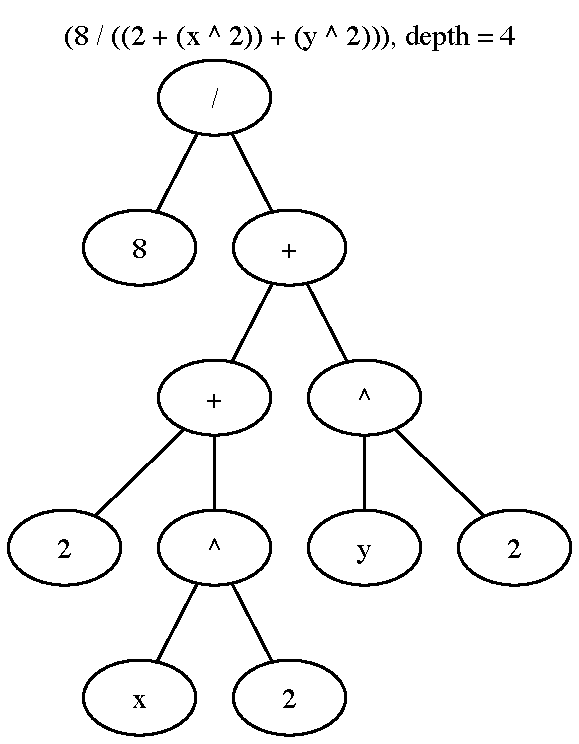
\includegraphics[width=\linewidth]{expression_tree_Hemberg2008_expr_1.pdf}
    \caption{Expression tree for expression 1 in Table \ref{tab:Hemberg2008PreIP_results}. The prefix form of the expression is \texttt{/ 8 + + 2 \^\ x 2 \^\ y 2} and the postfix form of the expression is \texttt{/ 8 + + 2 \^\ x 2 \^\ y 2}. }
    \label{fig:expression_tree_Hemberg2008_expr_1}
\end{figure}

\begin{figure}
    \centering
    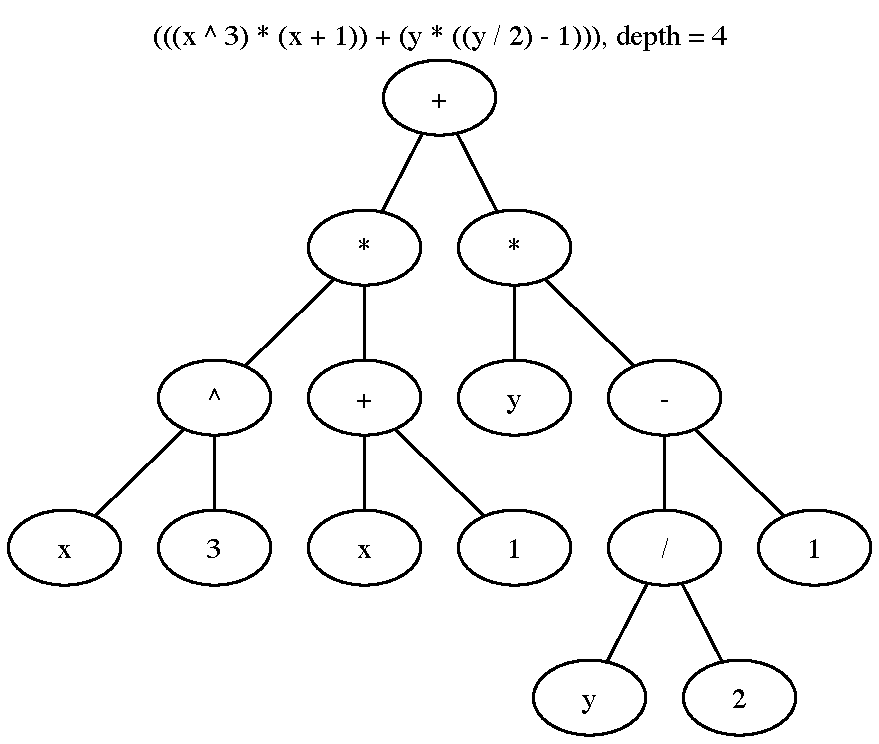
\includegraphics[width=\linewidth]{expression_tree_Hemberg2008_expr_2.pdf}
    \caption{Expression tree for expression 2 in Table \ref{tab:Hemberg2008PreIP_results}. The prefix form of the expression is \texttt{x 3 \^\ x 1 + * y y 2 / 1 - * +} and the postfix form of the expression is \texttt{x 3 \^\ 5 / y 3 \^\ 2 / + y - x -}. } 
    \label{fig:expression_tree_Hemberg2008_expr_2}
\end{figure}

\begin{figure}
    \centering
    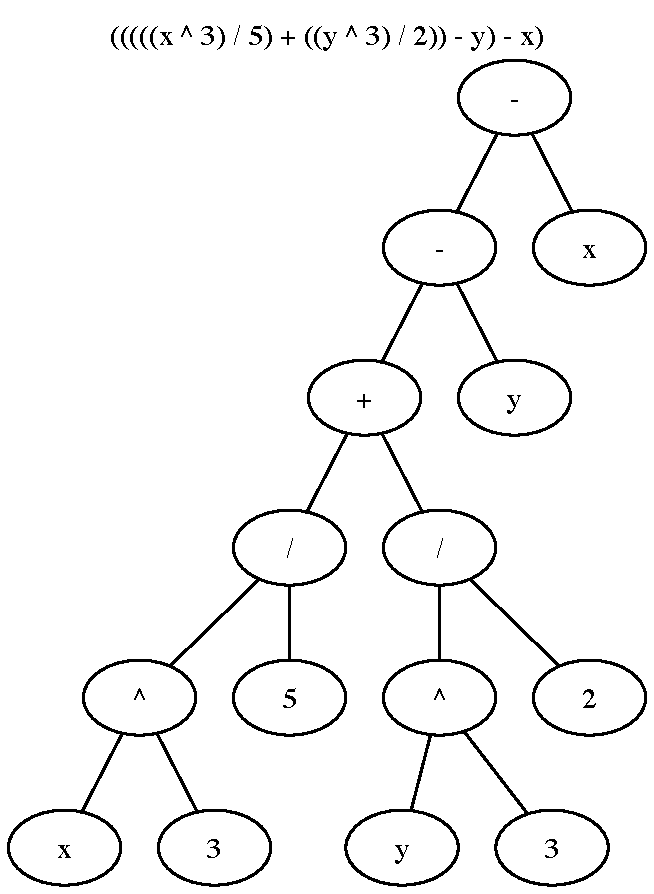
\includegraphics[width=\linewidth]{expression_tree_Hemberg2008_expr_3.pdf}
    \caption{Expression tree for expression 3 in Table \ref{tab:Hemberg2008PreIP_results}. The prefix form of the expression is \texttt{ - - + / \^\ x 3 5 / \^\ y 3 2 y x} and the postfix form of the expression is \texttt{x 3 \^\ 5 / y 3 \^\ 2 / + y - x -}. } 
    \label{fig:expression_tree_Hemberg2008_expr_3}
\end{figure}

\begin{figure}
    \centering
    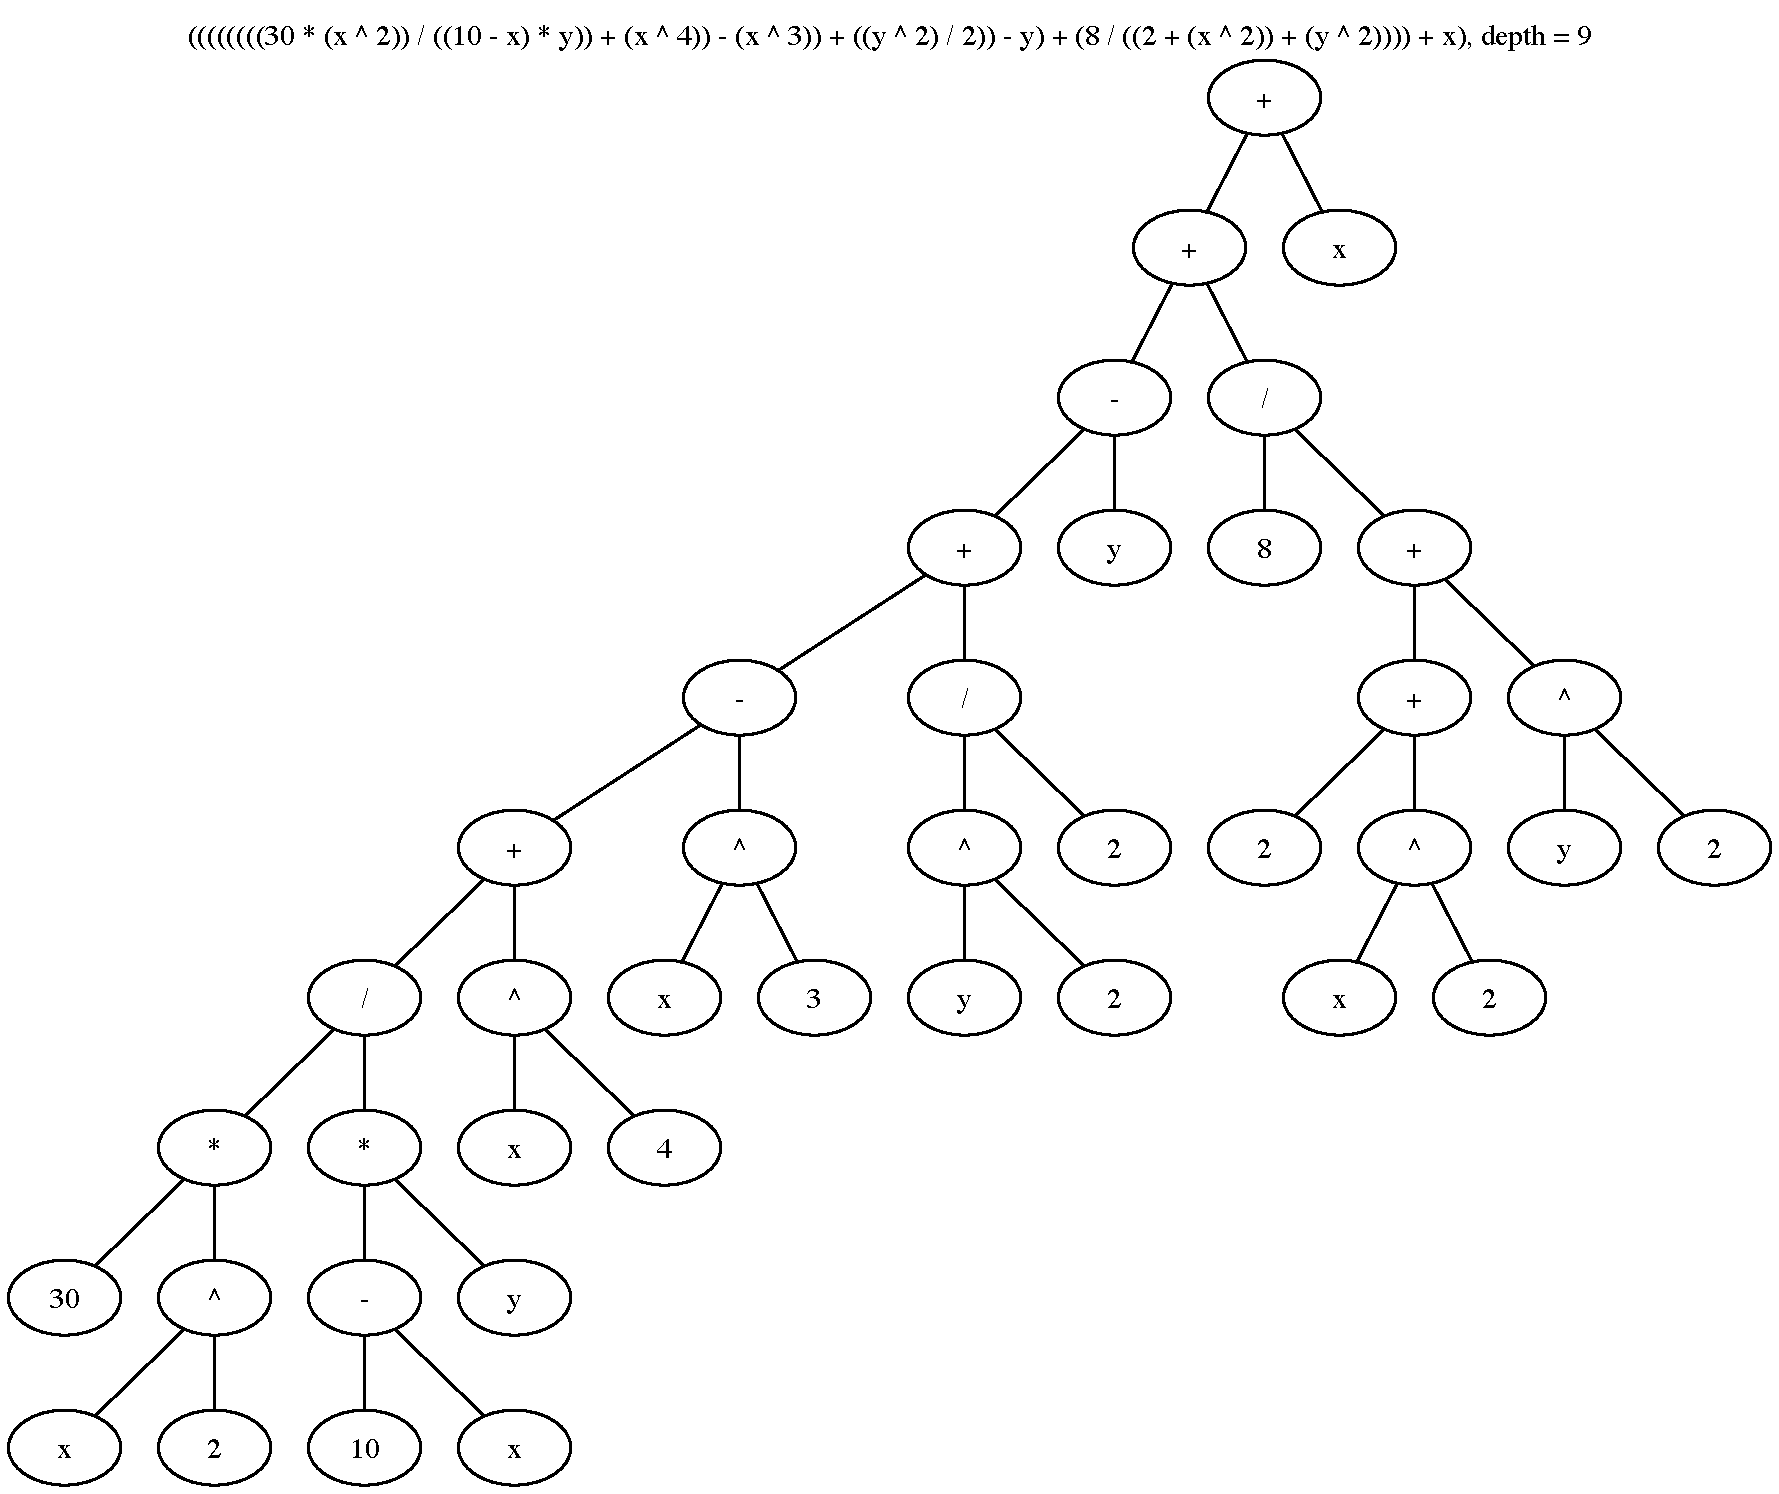
\includegraphics[width=\linewidth]{expression_tree_Hemberg2008_expr_4.pdf}
    \caption{Expression tree for expression 4 in Table \ref{tab:Hemberg2008PreIP_results}.  The prefix form of the expression is \texttt{+ + - + - + / * 30 \^\ x 2 * - 10 x y \^\ x 4 \^\ x 3 / \^\ y 2 2 y / 8 + + 2 \^\ x 2 \^\ y 2 x} and the postfix form of the expression is \texttt{30 x 2 \^\ * 10 x - y * / x 4 \^\ + x 3 \^\ - y 2 \^\ 2 / + y - 8 2 x 2 \^\ + y 2 \^\ + / + x +}. } 
    \label{fig:expression_tree_Hemberg2008_expr_4}
\end{figure}

\begin{figure}
    \centering
    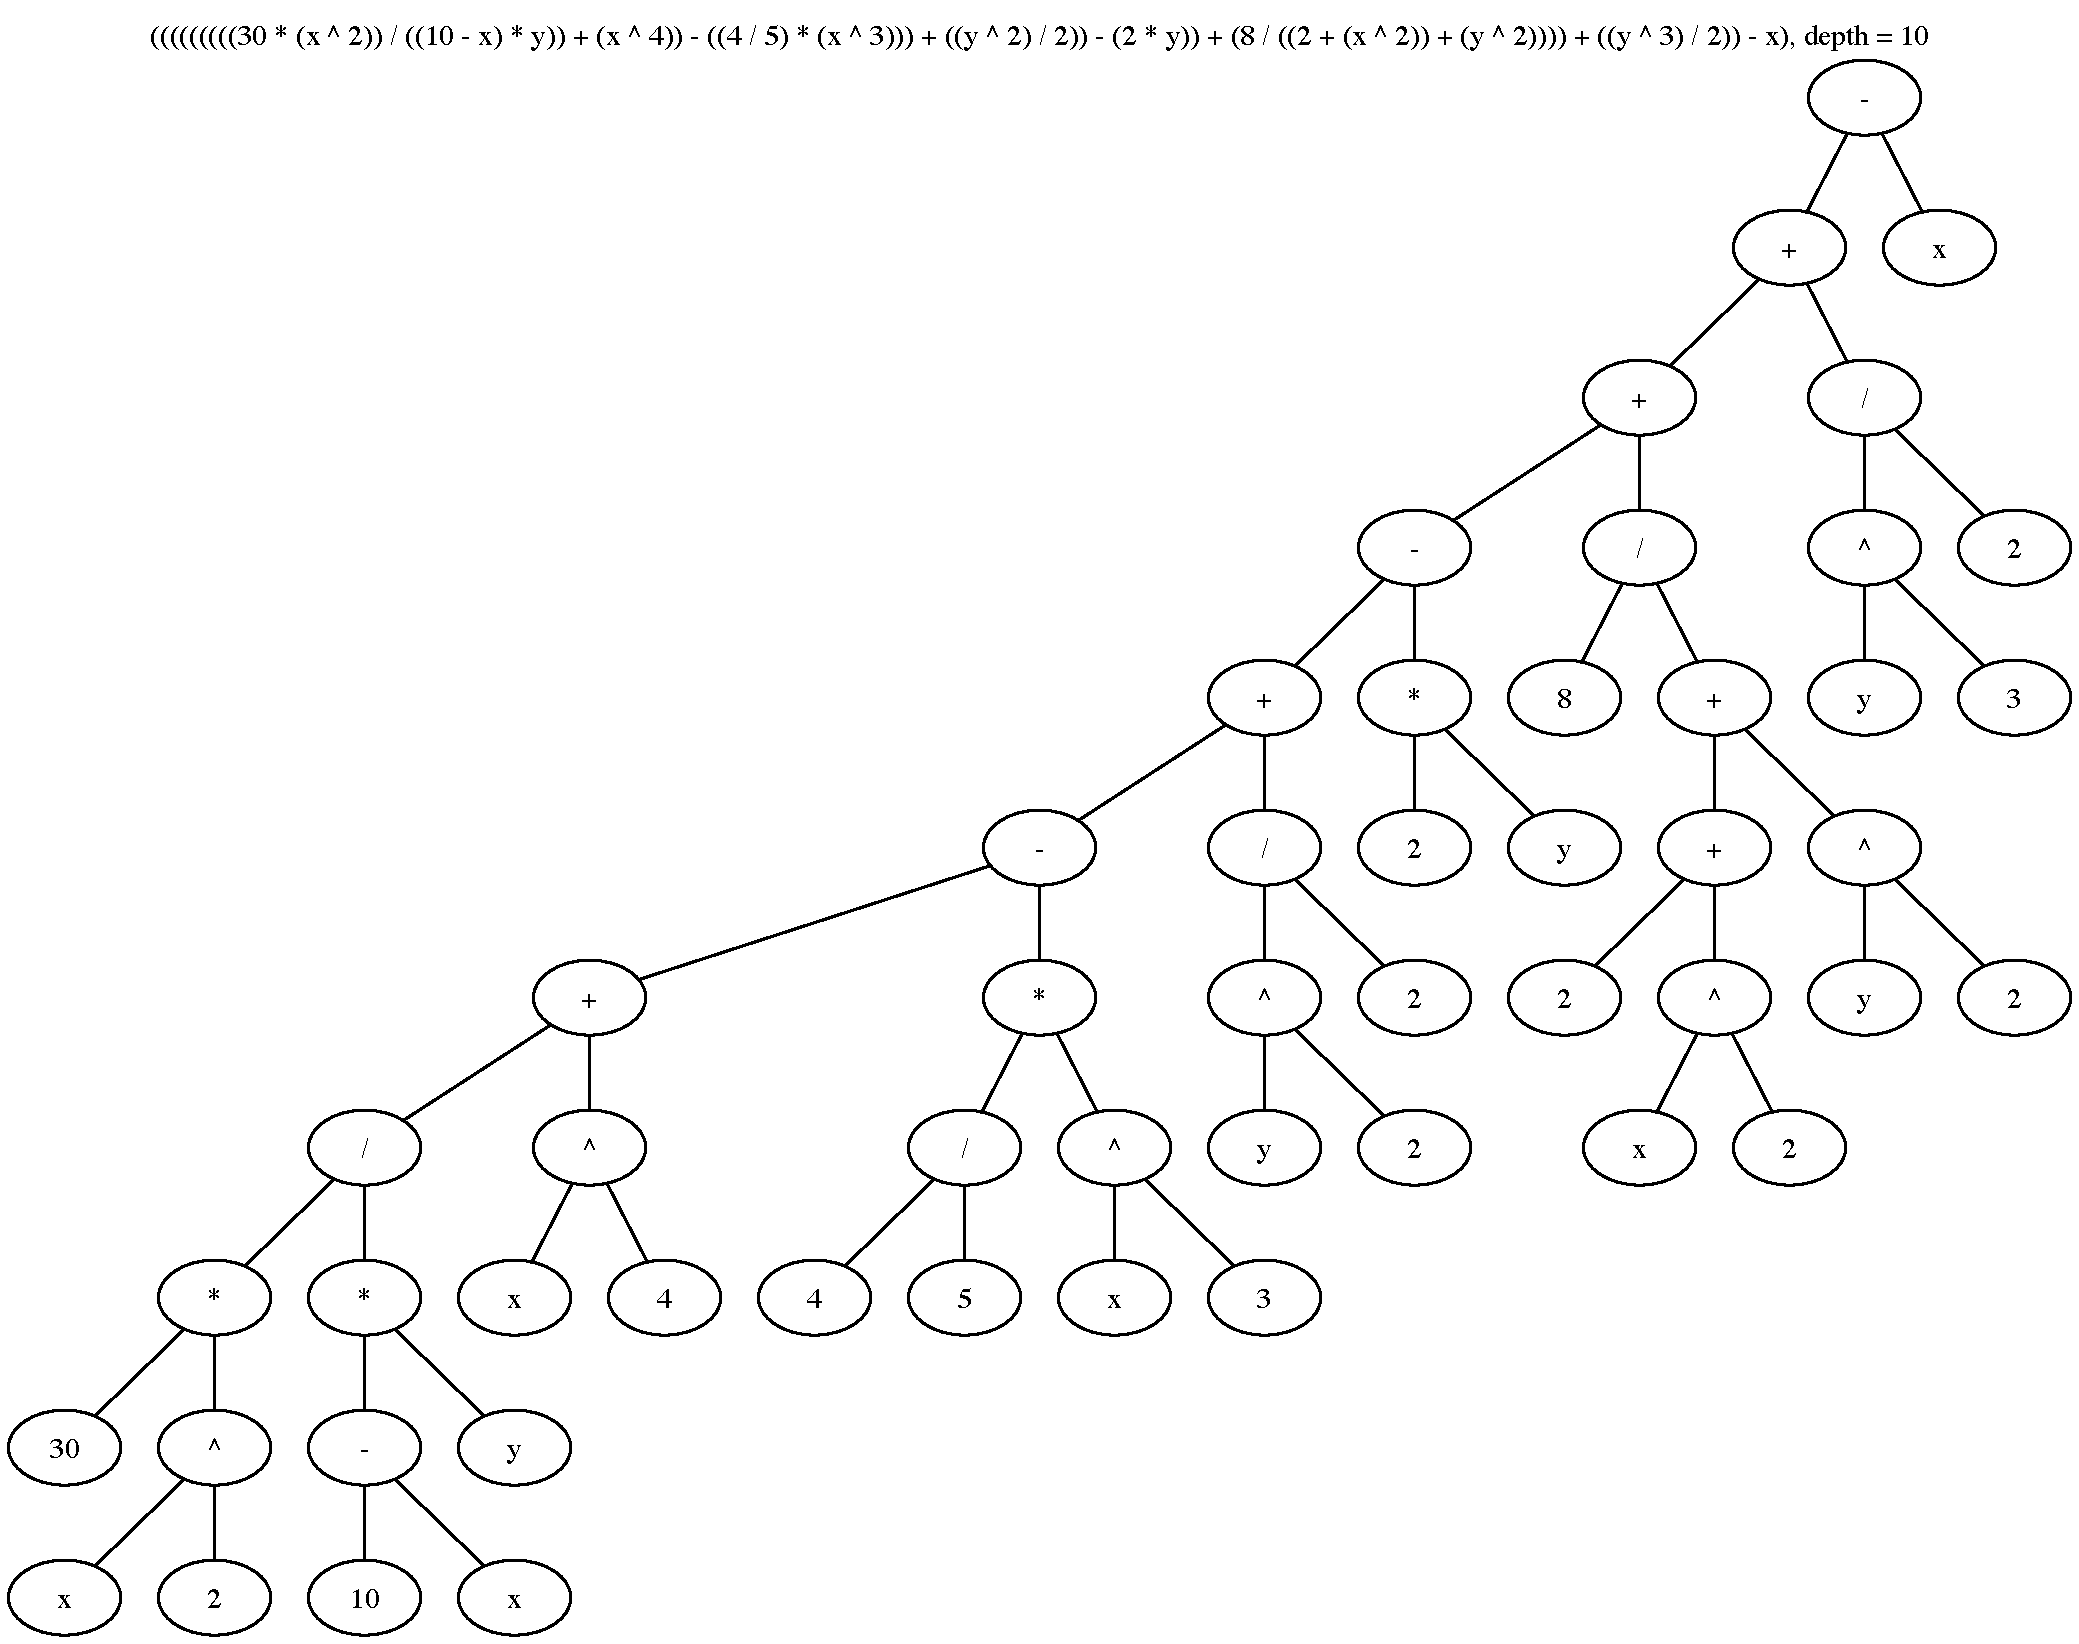
\includegraphics[width=\linewidth]{expression_tree_Hemberg2008_expr_5.pdf}
    \caption{Expression tree for expression 5 in Table \ref{tab:Hemberg2008PreIP_results}. The prefix form of the expression is \texttt{- + + - + - + / * 30 \^\ x 2 * - 10 x y \^\ x 4 * / 4 5 \^\ x 3 / \^\ y 2 2 * 2 y / 8 + + 2 \^\ x 2 \^\ y 2 / \^\ y 3 2 x} and the postfix form of the expression is \texttt{30 x 2 \^\ * 10 x - y * / x 4 \^\ + 4 5 / x 3 \^\ * - y 2 \^\ 2 / + 2 y * - 8 2 x 2 \^\ + y 2 \^\ + / + y 3 \^\ 2 / + x -}. } 
    \label{fig:expression_tree_Hemberg2008_expr_5}
\end{figure}


\end{document}

